% vi:ft=tex
\documentclass{standalone}

\usepackage{tikz}
\usepackage{verbatim}

\usetikzlibrary{arrows}
\usetikzlibrary{calc}

\begin{document}

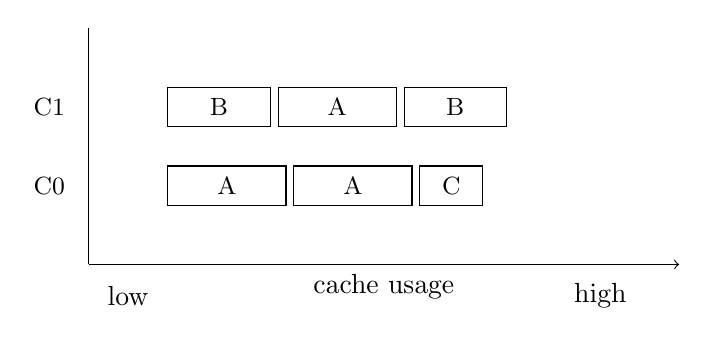
\begin{tikzpicture}

  % Colors
  % Styles
  \tikzstyle{defaultRec} = [font=\small, text centered, inner sep = 1pt,
    draw=black, shape=rectangle, fill=white, anchor=west, minimum height = .5cm];
  \tikzstyle{smallJob} = [defaultRec, minimum width = .5cm, minimum height =
  1cm];
  \tikzstyle{largeJob} = [defaultRec, minimum width = 1.3cm];
  \tikzstyle{mediumJob} = [defaultRec, minimum width = .8cm, minimum height =
  .7cm];

  \tikzstyle{defaultCirc} = [font=\small, text centered, inner sep = 1pt,
    draw=none, shape=circle];
  \tikzstyle{core} = [defaultCirc, minimum width = 1cm];

  \tikzstyle{timeArrow} = [->, thin, black];

  % Variables
  \newcommand\Ymax{3};
  \newcommand\Xmax{7};
  \newcommand\fstLvl{1};
  \newcommand\sndLvl{2};


% Drawing

  % balanced by time usage
  \begin{scope} []
    \tikzstyle{smallJobCache} = [defaultRec, minimum width = 1.5cm];
    \tikzstyle{mediumJob} = [defaultRec, minimum width = .8cm];

    \draw[timeArrow] (0,0) -- (7.5,0) node[below, text centered, midway]{cache usage};

    \node[draw=none] at (0.5 cm, -.4cm) {low};
    \node[draw=none] at (6.5 cm, -.4cm) {high};

    \draw[thin, black] (0,0) -- (0,\Ymax);

    \node(c1) [defaultCirc, minimum width = .5cm] at (-.5, \fstLvl) {C0};
    \node(c2) [defaultCirc, minimum width = .5cm] at (-.5, \sndLvl) {C1};

    %core 1
    \node[largeJob] at (1,\sndLvl) {B};
    \node[smallJobCache] at (2.4,\sndLvl) {A};
    \node[largeJob] at (4,\sndLvl) {B};

    % core 0
    \node[smallJobCache] at (1,\fstLvl) {A};
    \node[smallJobCache] at (2.6,\fstLvl) {A};
    \node[mediumJob] at (4.2, \fstLvl) {C};
  \end{scope}

\end{tikzpicture}

\end{document}
